\documentclass[12pt,fleqn]{article}\usepackage{../common}
\begin{document}
SVD ile Zaman Serisi Kumeleme

Ornek olarak [1] adresinde tarif edilen / paylasilan zaman serisini
kullandik. Once veriyi grafikledik, 

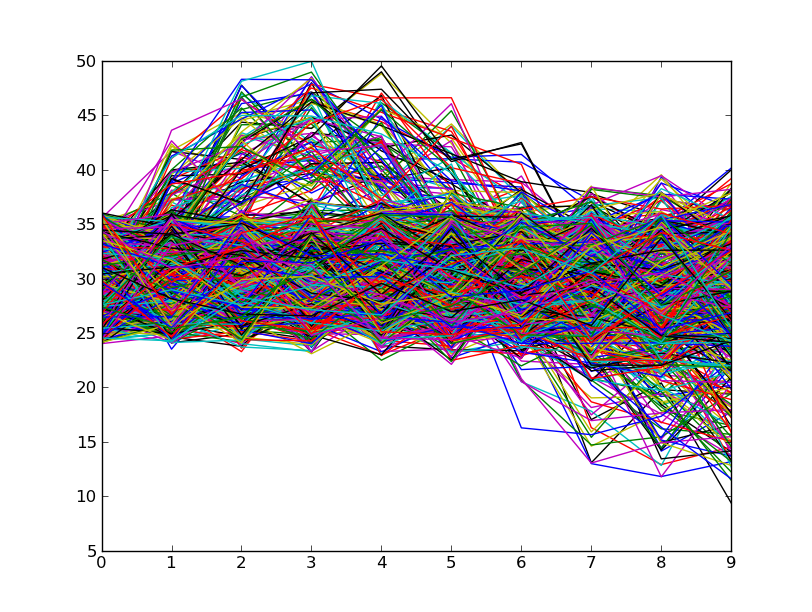
\includegraphics[height=4cm]{data.png}

Verinin tamami kullanilmadi, serinin ilk 10 noktasini aldik, 

\lstinputlisting[language=Python]{time1.py}

Grafige bakinca iki tane ana seri oldugunu goruyoruz. Peki bu serileri 

[1] http://kdd.ics.uci.edu/databases/synthetic\_control/synthetic\_control.data.html


\end{document}
